% ##################################################################################################################
\section{Cottbus: Traffic Light Simulation}
\label{ch:scenarios:cottbus}
\hfill \textbf{Authors:} Joschka Bischoff, Dominik Grether

\editdone{This text has undergone the professional edit. Please no grammatical changes anymore! They are most-probably wrong.}

% ##################################################################################################################
The Cottbus (Germany) scenario (Figure~\ref{fig:scenarios:cottbus_location}) is used for traffic light simulation (see Chapter~\ref{ch:signalslanes}). 
It is explained well in \citet[][pp.~87]{Grether_PhDThesis_2014}; this chapter briefly reviews the main points. 
The scenario data is generally available to the public.

The network is derived from \gls{osm} data in summer, 2010 \citep{Bischoff2010BaSylvia} and 
covers all streets within the city boundaries, as well as main roads in the surrounding Spree-Neiße administrative district . 
It is designed as a 100\,\% sample. 
The population is based on the German federal employment agency commuter statistics for both Cottbus and Spree-Neiße \citep{WiethoelterBogaiCarstensen2010IABPendlerberichtBB}. 
As such, the population has only home-work-home plans spread over the usual commuting times, resulting in two peaks, including 
33\,479 agents traveling exclusively by car. 
The scenario is generally not very busy; the area does not usually have major congestion issues.

Figure~\ref{fig:network_municipalities_cottbus_landuse} shows the network over the 
"Corine Land Cover" landuse \citep{CorineLandCover2006Data}, provided by European Environmental Agency. 
Woods and agricultural areas are depicted; most of the region is agricultural use area.  
Virtual persons in \gls{matsim} need a geographic coordinate for their activities. 
If this coordinate is drawn randomly (solely based on municipality borders), home and work activity locations are uniformly distributed over  the area, i.e.,\,most of them in woods and fields. 
Thus, activity locations are drawn randomly in combination with land use data. 
The coordinate must be in the municipality area and for home activity, it must be located in urban fabric areas; for work locations, industrial or commercial areas are also allowed. 
The resulting home activity locations are shown in Figure~\ref{fig:cottbus_population_home}. 

The scenario contains data for 22\,traffic signals within the city center, based on the city's 2009 signal plans; junction layout is also modeled in detail. Fixed-time control data is taken from \citet{KoehlerStrehler2010SignalDemandOptimization}.  
Due to higher transport network resolution, several originally recorded fixed-time control schedules are invalid and were removed; data for 22\,junctions is available. 
Figure~\ref{fig:cottbus_network_signal_locations} shows their transport network location.  

Public transit, not part of the original scenario, is available based on 2011 schedules, although it is not currently used. 
\createfigure%
{Cottbus Scenario: Geospatial location within Germany, Europe}%
{Cottbus Scenario: Geospatial location within Germany, Europe}%
{\label{fig:scenarios:cottbus_location}}%
{%
  \createsubfigure%
	{Geospatial area of Brandenburg within Germany, Europe (Red); City of Berlin (Yellow)}
	{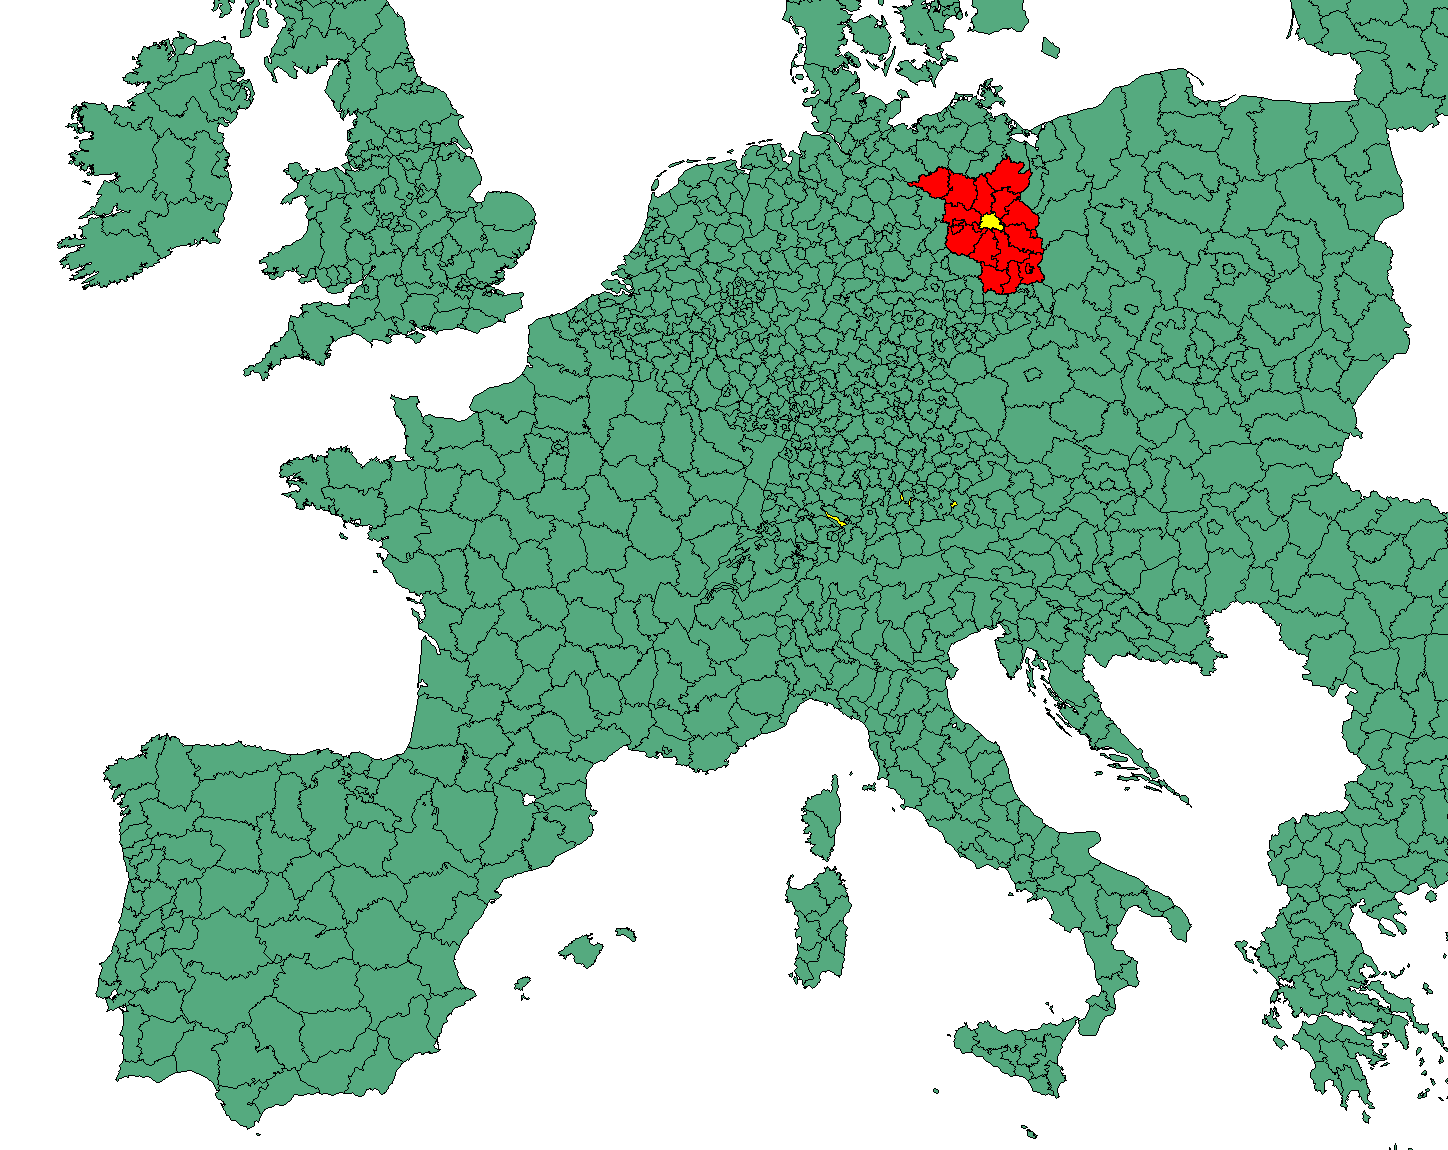
\includegraphics[width=0.49\textwidth]{./using/figures/brandenburg_europe.png}}
	{\label{fig:scenarios:cottbus_brandenburg_europe}}
  \createsubfigure%
	{Geospatial area of Cottbus (Dark Red), within administrative district Spree-Neiße, Brandenburg (Light Red)}
	{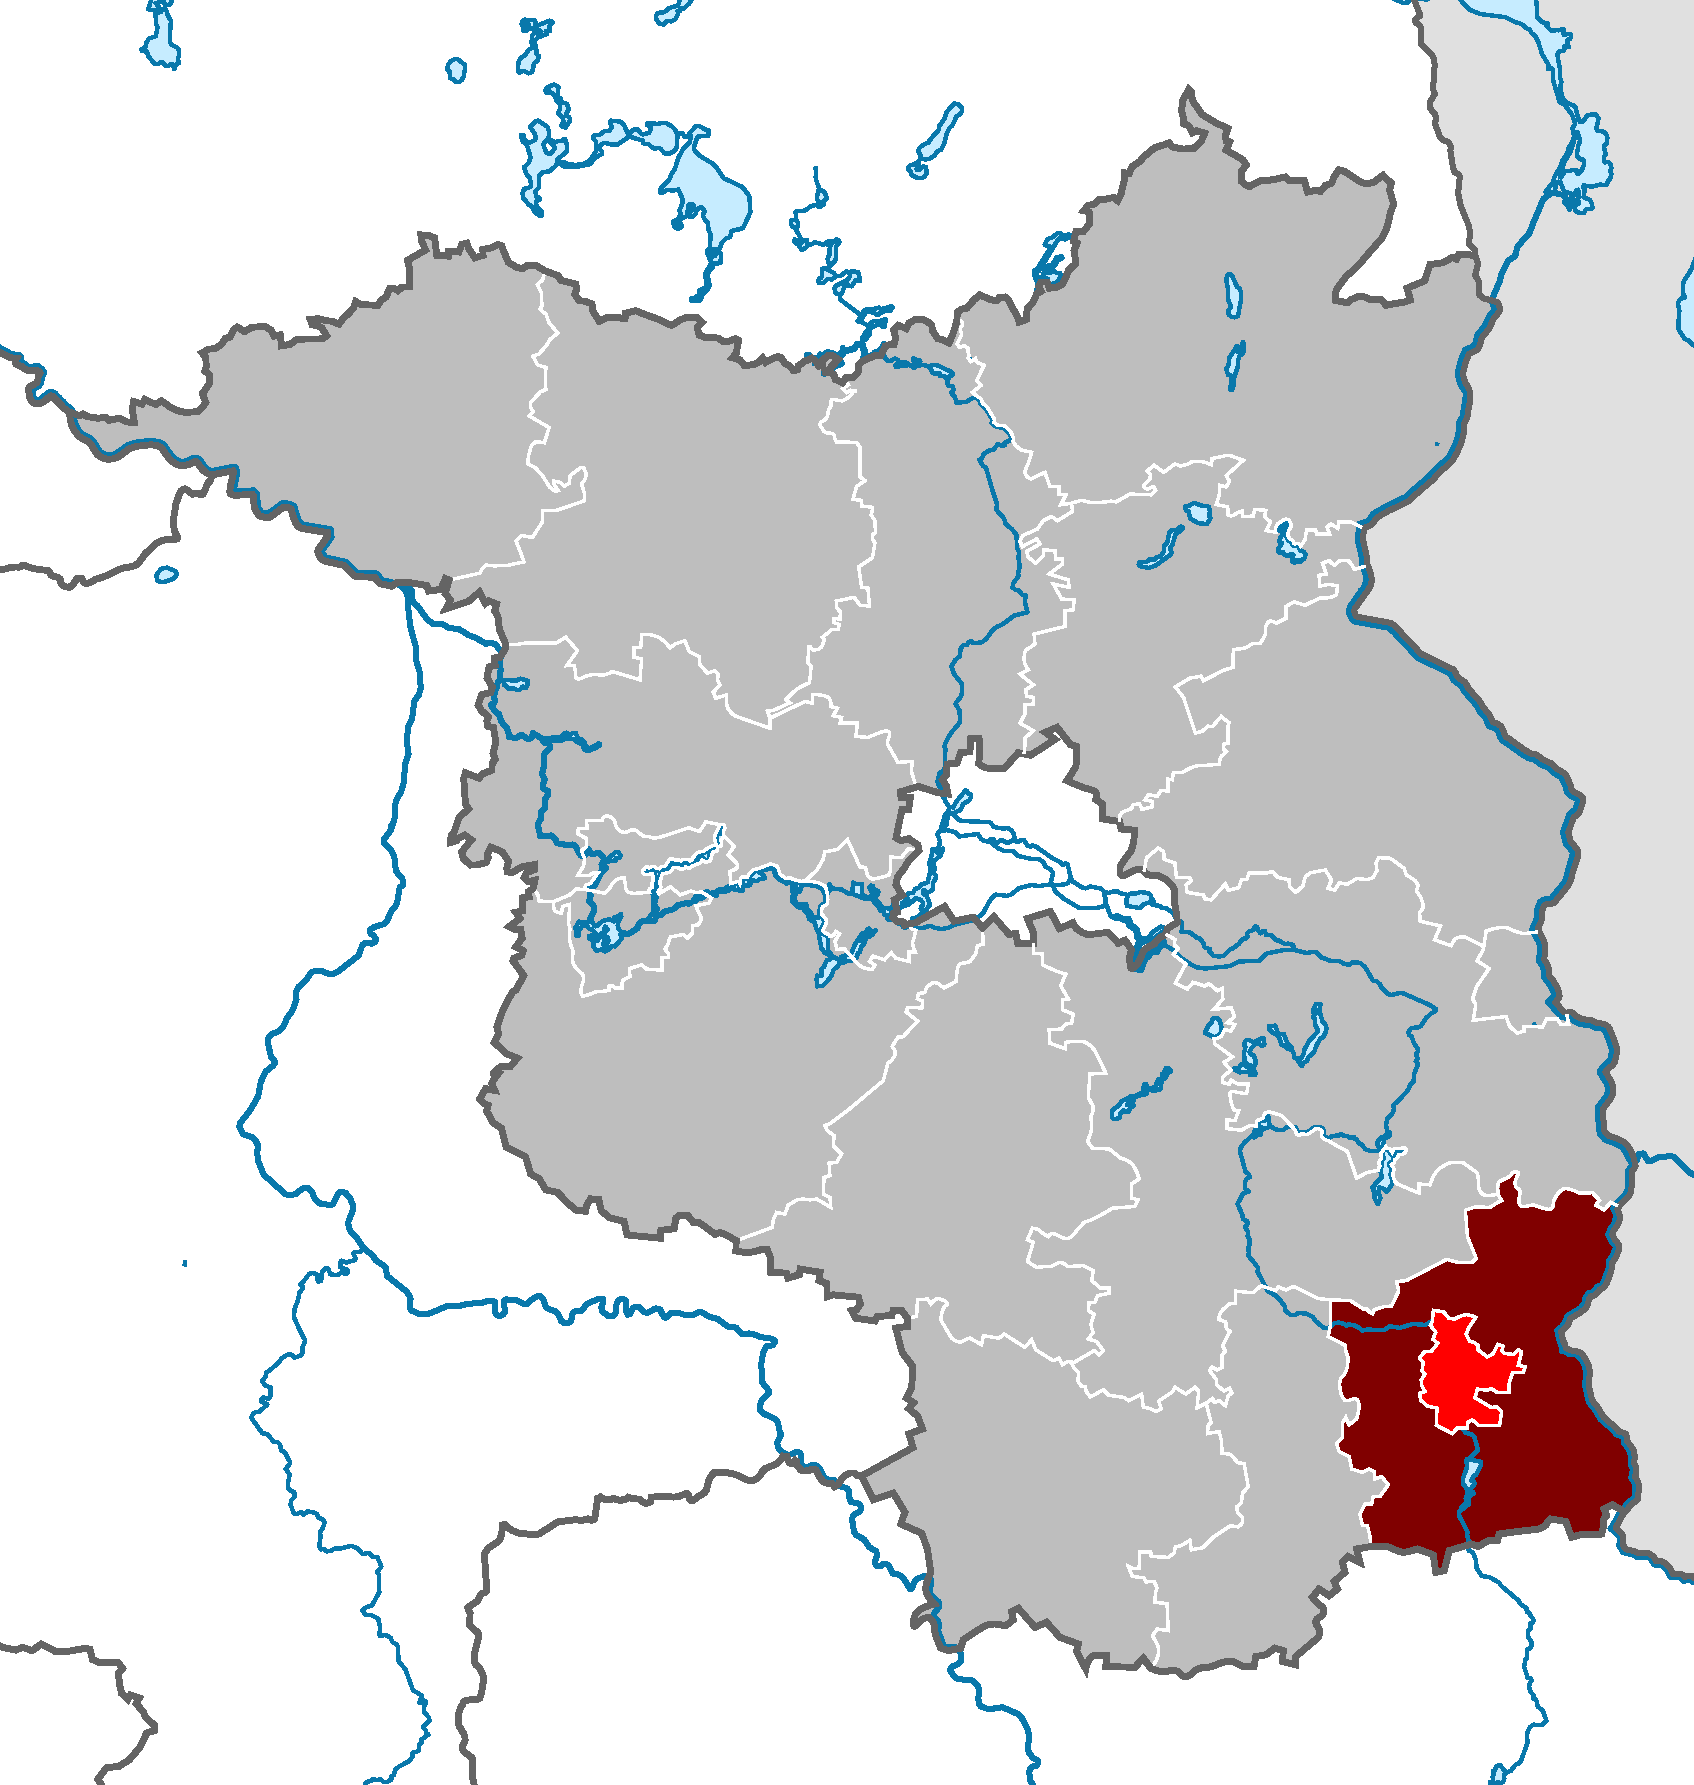
\includegraphics[width=0.49\textwidth]{./using/figures/brandenburg_spree_neise_cottbus.pdf}}
	{\label{fig:scenarios:cottbus_bb}}
}%
{\citet{Grether2014PhD}}

\createfigure%
{Cottbus Scenario: Network and Population}%
{Cottbus Scenario: Network and Population}%
{\label{fig:cottbus_network_population}}%
{%
  \createsubfigure%
	{Cottbus network and municipality borders}
	{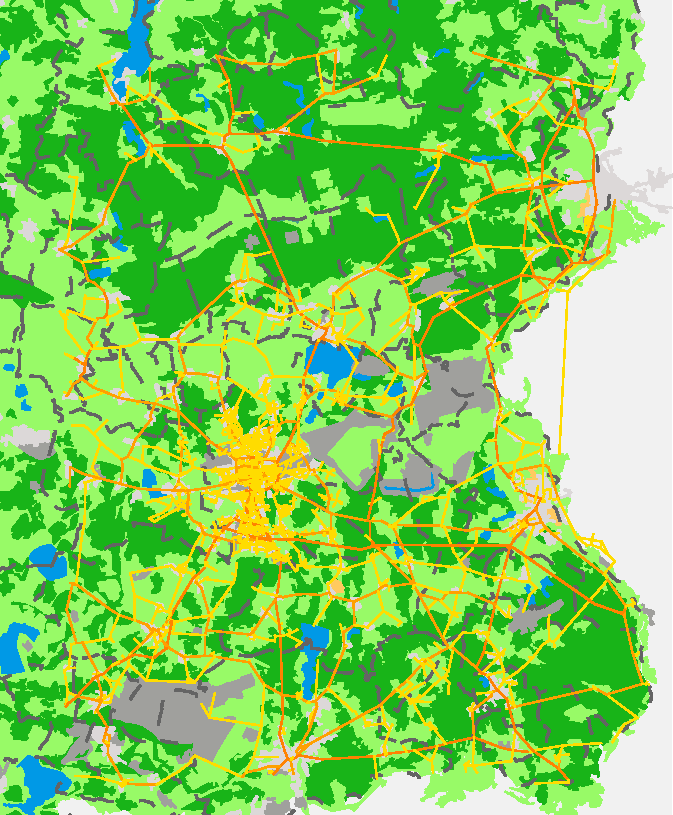
\includegraphics[width=0.49\linewidth]{./using/figures/2013_network_gemeinden_landuse_edit.pdf}}
	{\label{fig:network_municipalities_cottbus_landuse}}
  \createsubfigure%
	{Synthetic population for the Cottbus scenario, geospatial location of home activities}
	{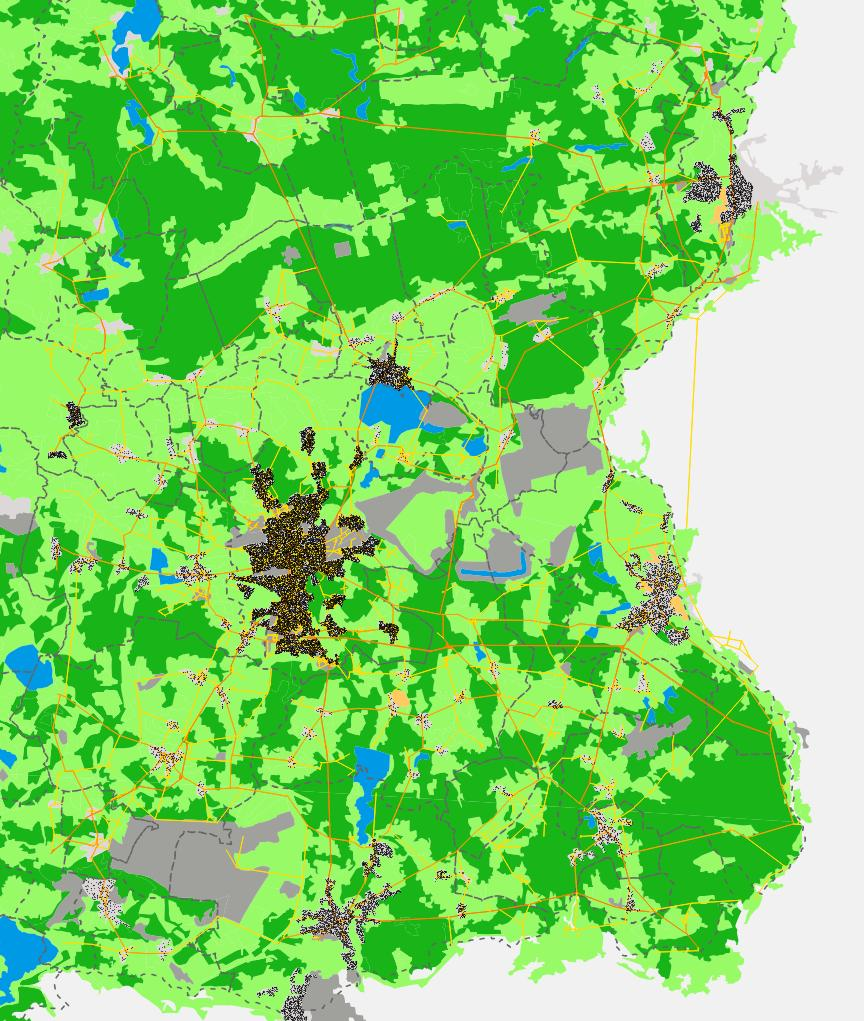
\includegraphics[width=0.49\linewidth]{./using/figures/2013_network_gemeinden_landuse_population_home.jpg}}
	{\label{fig:cottbus_population_home}}
}%
{Source:~\citet{Grether2014PhD}} 

\createfigure%
{Cottbus scenario: Network, area with traffic signals within the city of Cottbus}
{Cottbus scenario: Network, area with traffic signals within the city of Cottbus}
{\label{fig:cottbus_network_signal_locations}}
{%
  \createsubfigure%
	{Location within city of Cottbus}
	{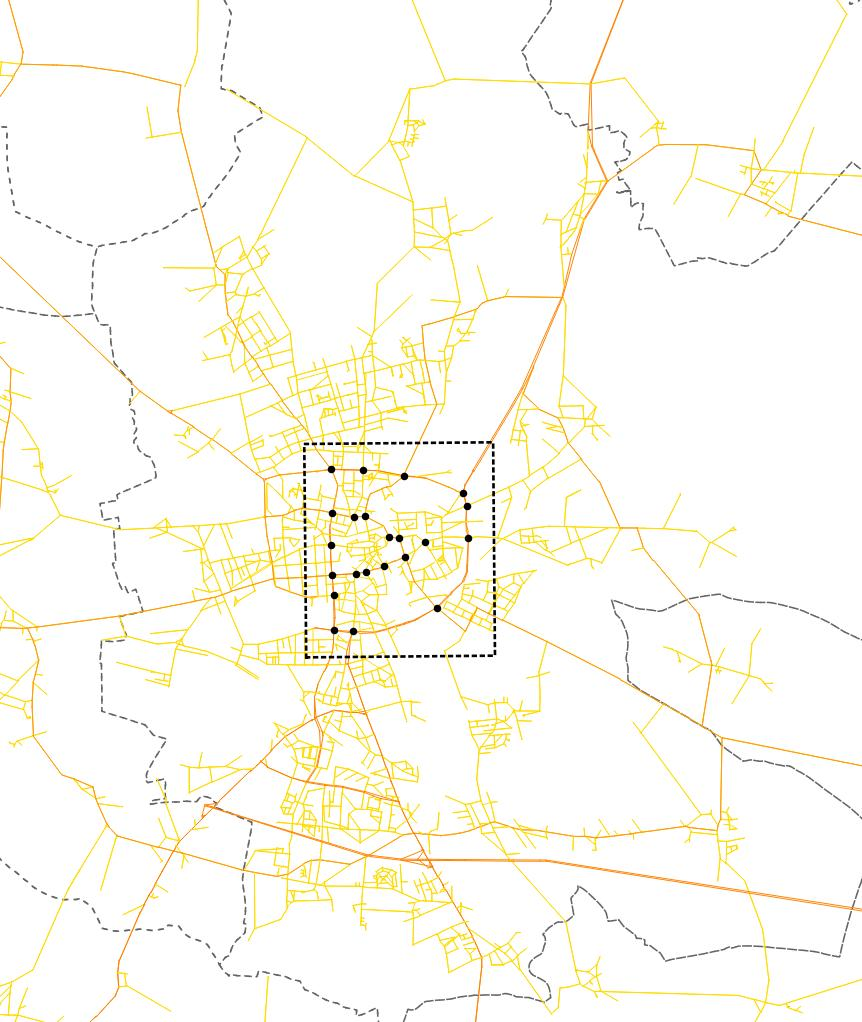
\includegraphics[width=0.49\linewidth]{./using/figures/2013_cottbus_network_signals.jpg}}
	{\label{fig:cottbus_network_signals}}
  \createsubfigure%
	{Signalized area in detail}
	{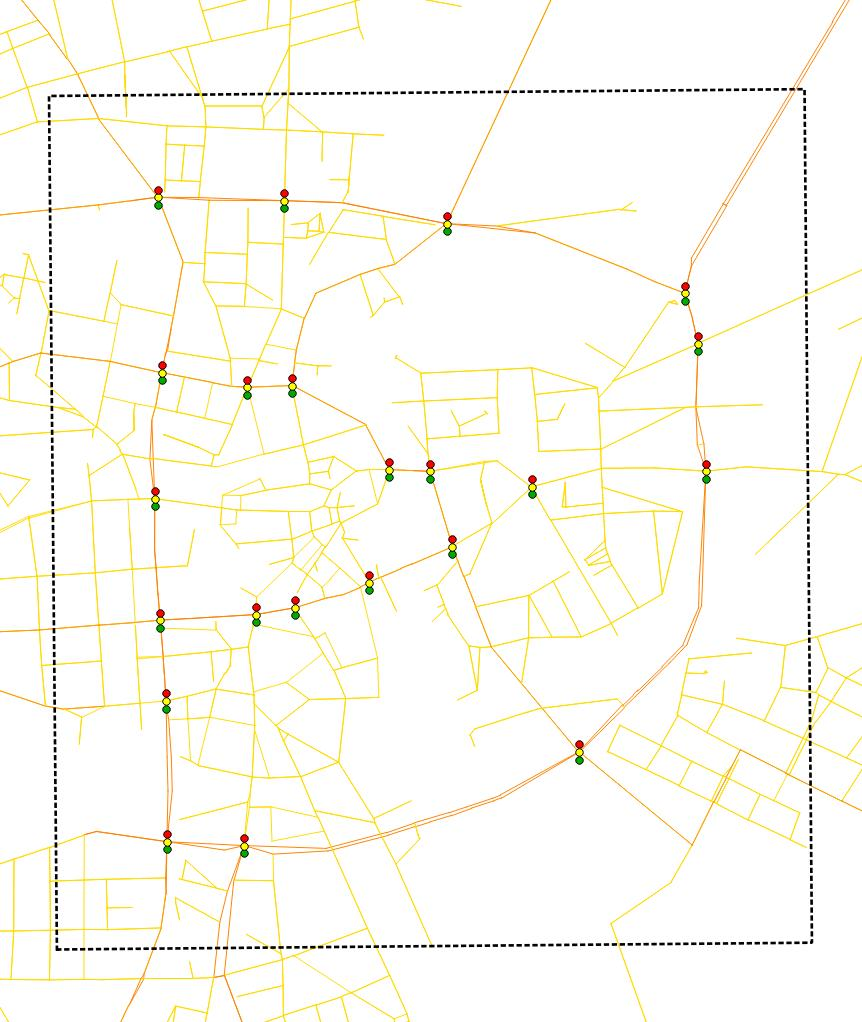
\includegraphics[width=0.49\linewidth]{./using/figures/2013_cottbus_network_signals_zoom.jpg}}
	{\label{fig:cottbus_network_signals_zoom}}
}%
{\citet{Grether2014PhD}}

% ##################################################################################################################

% Andreas Neumann-Mail: frei verfügbar. ÖV vorhanden, 100\% Szenario, das sich mit einigermassen geringem Aufwand rechnen lässt. Grundlage für Dominik G.s Ampelpart
